\chapter[Stima Fatturato]{Stima Fatturato}
La stima sul potenziale fatturato che potremmo realizzare in ogni mese è stato calcolato precisamente analizzando durante l'anno 2016:
\begin{itemize}
	\item il numero di potenziali clienti interessati dalla nostra offerta;
	\item il volume di traffico di chiamate generato da ogni singolo operatore;
\end{itemize}
Combinando opportunamente queste due stime possiamo calcolare facilmente i contratti stipulati e, quindi, i guadagni realizzati ogni mese.\newline
	\begin{tcolorbox}[colframe=blue!75!black,adjusted title=\textbf{Osservazione!}]
		Dai dati forniti da \textbf{Sistelia} abbiamo osservato che per ogni contratto realizzato con successo per conto di \textbf{ReteTurismo} il guadagno è di \euro \hspace{0,0150625cm} 80. 
	\end{tcolorbox}
\section[Numero Potenziali Viaggiatori]{Numero Potenziali Viaggiatori}
Per l'analisi dei dati relativi al numero dei potenziali clienti ci siamo ricavati questo valore dalla regressione dei dati forniti dall'istat nel periodo 2012-2015:
\begin{savenotes}
\begin{table}[htb]
\centering
 \caption{Numero Viaggi con pernottamento italiani}
 \begin{tabular}{p{3cm}D{,}{,}{5.2}}
 \toprule
 	\multicolumn{1}{c}{\textbf{Anno}} & \multicolumn{1}{c}{\textbf{\% viaggi con pernottamento }} \\
 \midrule 		
	\makebox[3cm][c]{2012} & 19,20\\
 	\makebox[3cm][c]{2013} & 18,10\\
 	\makebox[3cm][c]{2014} & 16,38\\  	
 	\makebox[3cm][c]{2015} & 16,50\\
 \bottomrule
 \end{tabular} 
\end{table}
\end{savenotes}

 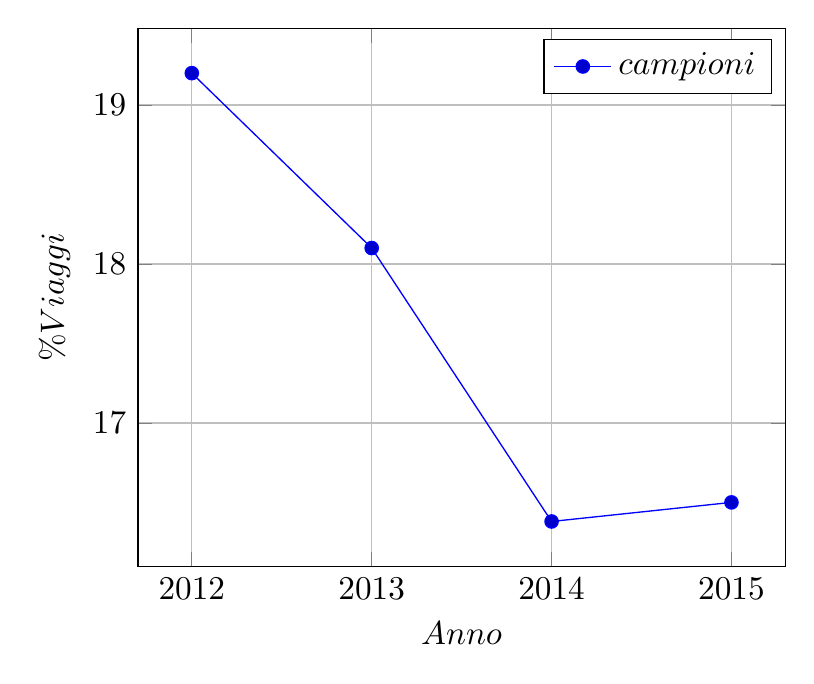
\begin{tikzpicture}[scale=1.2]
 \pgfkeys {
			/pgf/number format/.cd,
			set decimal separator={,{\!}},
			set thousands separator={}}
	\begin{axis}[ xlabel=$Anno$, ylabel=$\% Viaggi$, grid=major,
	xtick= {2012,2013,2014,2015} ]
		
		\addplot coordinates{( 2012, 19.20) 
							  ( 2013, 18.10)
							  ( 2014, 16.38)
							  ( 2015, 16.50)
							  };
				\legend{$campioni$,$regressione$}
	\end{axis}
\end{tikzpicture}

per ottenere il valore relativo all'anno 2016 è stata calcolata la \textit{funzione di regressione} sui dati precedenti:
\newline
	\begin{equation}
	\label{eq:reg_num_viaggi}
	\begin{split}
		y(x) = -2,16322 \cdot ln( 1,35775 \cdot 10^{-4} \cdot x)
	\end{split}
	\end{equation}

 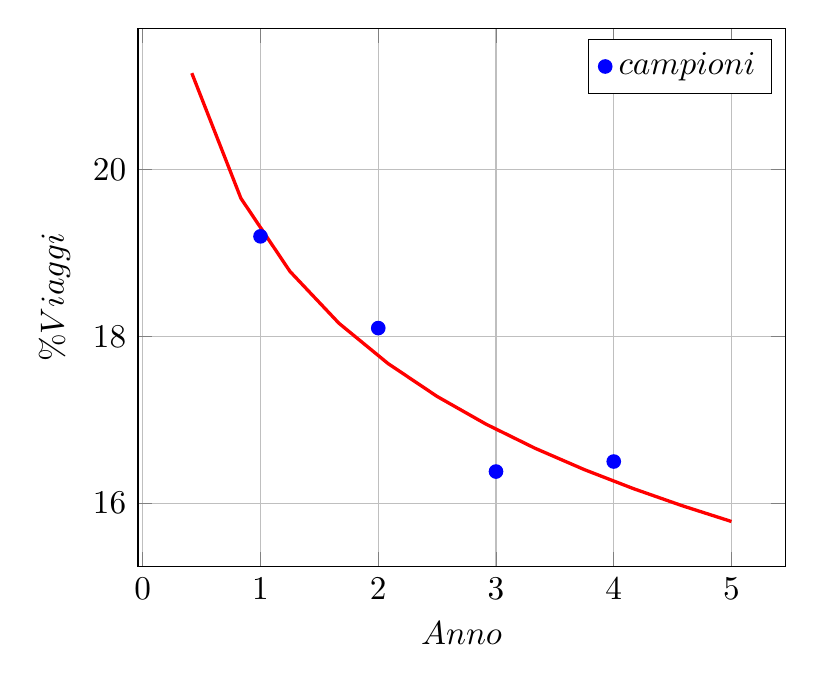
\begin{tikzpicture}[scale=1.2]
 \pgfkeys {
			/pgf/number format/.cd,
			set decimal separator={,{\!}},
			set thousands separator={}}
	\begin{axis}[ xlabel=$Anno$, 
				   ylabel=$\% Viaggi$, 
				   grid=major]
		


		\addplot [color=blue, only marks]coordinates{( 1.0, 19.20) 
							  ( 2.0, 18.10)
							  ( 3.0, 16.38)
							  ( 4.0, 16.50)
							  };
				

		\addplot[color=red, line width=1pt]{-2.16322 * ln( 1.35775 * 10^(-4) * x)};
		
		\legend{$campioni$}
	\end{axis}
\end{tikzpicture}

La funzione \ref{eq:reg_num_viaggi} presenta, in particolare le seguenti caratteristiche:
\begin{savenotes}
\begin{table}[htb]
\centering
 \caption{Caratteristiche Funzione di Regressione}
 \begin{tabular}{p{3cm}D{,}{,}{7.5}}
 \toprule
 	\multicolumn{1}{c}{\textbf{Parametro}} & \multicolumn{1}{c}{\textbf{Valore}} \\
 \midrule 		
	\makebox[3cm][c]{\textbf{AIC}\footnote{\textit{\textbf{A}kaike's \textbf{I}nformation \textbf{C}riterion} è un metodo di valutazione e il confronto tra modelli statistici}} & 8,42376\\
 	\makebox[3cm][c]{\textbf{BIC}\footnote{\textit{\textbf{B}ayesian \textbf{I}nformation \textbf{C}riterion} è un criterio per la selezionedi un modello tra una classe di modelli parametrici}} & 6,58264\\
 	\makebox[3cm][c]{\textbf{$(R^{2})$}\footnote{varianza campionaria}} & 0,99965\\  	
 	\makebox[3cm][c]{\textbf{adjusted $(R^{2})$}\footnote{varianza campionaria corretta}} & 0,99931\\
 \bottomrule
 \end{tabular} 
\end{table}
\end{savenotes}



in particolare, il dato ricercato è pari a:
\newline
\[ y(5) = 15,6 \]

	\begin{tcolorbox}[colframe=blue!75!black,adjusted title=\textbf{Osservazione!}]
		Si calcola il valore della funzione \ref{eq:reg_num_viaggi} nel punto \[x = 5\] perchè il 2016 rappresenterebbe il quinto elemento nella serie di dati considerati
	\end{tcolorbox}
\section[Volume Traffico Generato Dipendenti]{Volume Traffico Generato Dipendenti}
Dai dati forniti da varie fonti di call center abbiamo stimato che il \textbf{tempo medio di una chiamata} (compresa di digitazione e attesa) è pari a:
	\begin{equation}
	\label{eq:durata_media_chiamate}
	\begin{split}
		3 \: minuti \: e \: 30 \: secondi \: = \: 3,5 \: minuti  
	\end{split}
	\end{equation}
Considerando, quindi, che in una giornata un operatore è al lavoro per circa:
	\begin{equation}
	\label{eq:durata_orario_lavoro}
	\begin{split}
		5 \: ore \: e \: 30 \: minuti \: = \: 5,5 \: ore  
	\end{split}
	\end{equation}
Possiamo stimare che in una giornata un centralinista è in grado di effettuare un numero di chiamate pari a:
	\begin{equation}
	\label{eq:num_chiamate_singolo_operatore_giorno}
	\begin{split}
		\frac{60}{3,5} \cdot 5,5 = 94,27 \simeq 94 
	\end{split}
	\end{equation}
se un anno lavorativo è costituito da 222 giorni effettivi, allora in un anno ogni singolo operatore è in grado di generare un flusso di chiamate pari a:
	\begin{equation}
	\label{eq:num_chiamate_singolo_operatore_anno}
	\begin{split}
		94 \cdot 222 = 20\thinspace 868 
	\end{split}
	\end{equation}
in totale, quindi tutti i dipendenti (30) generano (in un anno) un traffico pari a:
	\begin{equation}
	\label{eq:num_chiamate_azienda_anno}
	\begin{split}
		20\thinspace 868 \cdot 30 = 624\thinspace 040 
	\end{split}
	\end{equation}
\section[Fatturato Mensile]{Fatturato Mensile}
Dai dati stimati in precedenza, in particolare
\newline
\begin{center}
	\begin{tabular}{rr}
		numero di chiamate azienda annuali & 624\thinspace 040,00 \\
		tasso di successo viaggio (\%) & 15,60 \\
		tasso di successo firma contratto (\%) & 15,00 \\	
	\end{tabular}
\end{center}
possiamo determinare:
\begin{itemize}
\item il \textbf{numero medio contratti stipulati in un anno}
	\begin{equation}
	\label{eq:num_contratti_teorico_anno}
	\begin{split}
		\underbrace{624\thinspace 040 \cdot 0,1560}_{numero\: di\: clienti\: stipulano \: contratto \: viaggio } = 97\thinspace 350,24
	\end{split}
	\end{equation}

\item il \textbf{numero medio contratti stipulati in un anno (realistico)}
	\begin{equation}
	\label{eq:num_contratti_realistico_anno}
	\begin{split}
		\underbrace{\underbrace{624\thinspace 040 \cdot 0,1560 \cdot 0,15}_{numero\: clienti\: interessati \: viaggio } \cdot 0,15}_{numero \: clienti \: stipulano \: contratto} = 14\thinspace 602,54
	\end{split}
	\end{equation}

\item il \textbf{fatturato annuale}
	\begin{equation}
	\label{eq:fatturato_teorico_anno_netto}
	\begin{split}
		97\thinspace 350,24 \cdot 80,00 = 7\thinspace 788\thinspace 019,20 \: \mbox{\euro} 
	\end{split}
	\end{equation}	
	
\item il \textbf{fatturato annuale (realistico)}
	\begin{equation}
	\label{eq:fatturato_anno_netto}
	\begin{split}
		14\thinspace 602,54 \cdot 80,00 = 1\thinspace 168\thinspace 202,88 \: \mbox{\euro} 
	\end{split}
	\end{equation}

\item il \textbf{fatturato mensile}
	\begin{equation}
	\label{eq:fatturato_teorico_anno_netto}
	\begin{split}
		\frac{7\thinspace 788\thinspace 019,20 \: \mbox{\euro}}{12} = 649\thinspace 001,60 \: \mbox{\euro} 
	\end{split}
	\end{equation}	

	
\item il \textbf{fatturato mensile (realistico)} 
	\begin{equation}
	\label{eq:fatturato_mensile_netto}
	\begin{split}
		\frac{1\thinspace 168\thinspace 202,88}{12} = 97\thinspace 350,24 \: \mbox{\euro}
	\end{split}
	\end{equation}
	
\end{itemize}